\textbf{Результат работы.}

\begin{figure}[ht!]
	\centering{
		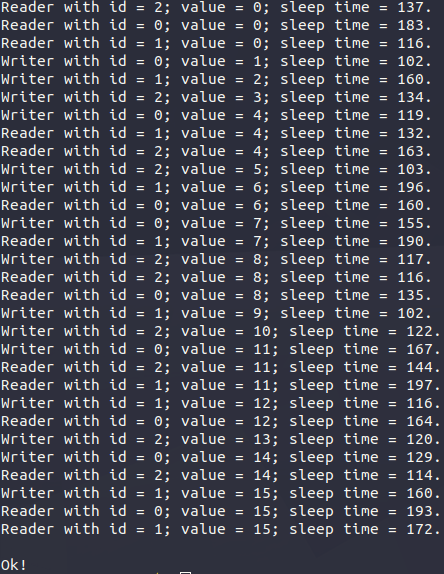
\includegraphics[width=1\textwidth]{img/res.png}
		\caption{Результат работы программы.} }
\end{figure}


\newpage

\begin{lstlisting}[label=some-code,caption=Код программы]
#include <windows.h>
#include <stdbool.h>
#include <stdio.h>
#include <time.h>
#include <stdbool.h>

#define OK 0

#define CREATE_MUTEX_ERROR 1
#define CREATE_EVENT_ERROR 2
#define CREATE_READER_THREAD_ERROR 3
#define CREATE_WRITER_THREAD_ERROR 3

#define MINIMUM_READER_DELAY 100
#define MINIMUM_WRITER_DELAY 100
#define MAXIMUM_READER_DELAY 200
#define MAXIMUM_WRITER_DELAY 200

#define READERS_NUMBER 3
#define WRITERS_NUMBER 3

#define ITERATIONS_NUMBER 5

HANDLE canRead;
HANDLE canWrite;
HANDLE mutex;

LONG waitingWritersCount = 0;
LONG waitingReadersCount = 0;
LONG activeReadersCount = 0;
bool writing = false;

HANDLE readerThreads[READERS_NUMBER];
HANDLE writerThreads[WRITERS_NUMBER];

int readersID[READERS_NUMBER];
int writersID[WRITERS_NUMBER];

int readersRand[READERS_NUMBER * ITERATIONS_NUMBER];
int writersRand[READERS_NUMBER * ITERATIONS_NUMBER];

int value = 0;

bool turn(HANDLE event)
{
	// Если функция возвращает WAIT_OBJECT_0, объект свободен.
	return WaitForSingleObject(event, 0) == WAIT_OBJECT_0;
}

void StartRead()
{
	// Увеличиваем кол-во ждущих читателей.
	InterlockedIncrement(&waitingReadersCount);

	// Процесс читатель сможет начать работать,
	// Если есть нет активного писателя,
	// И нет писателей, ждущих свою очередь.
	if (writing || turn(canWrite))
		WaitForSingleObject(canRead, INFINITE);

	WaitForSingleObject(mutex, INFINITE);
	// Уменьшаем кол-во ждущих читателей.
	InterlockedDecrement(&waitingReadersCount);
	// Увеличиваем кол-во активных читателей.
	InterlockedIncrement(&activeReadersCount);
	// Выдаем сигнал canRead,
	// Чтобы следующий читатель в очереди
	// Читателей смог начать чтение
	SetEvent(canRead);
	ReleaseMutex(mutex);
}

void StopRead()
{
	// Уменьшаем количество активных читателей.
	InterlockedDecrement(&activeReadersCount);
	// Если число читателей равно нулю,
	// Выполняется signal(can_write),
	// активизирующий писателя из очереди писателей.
	if (!activeReadersCount)
		SetEvent(canWrite);
}

DWORD WINAPI Reader(CONST LPVOID param)
{
	int id = *(int *)param;
	int sleepTime;
	int begin = id * ITERATIONS_NUMBER;
	for (int i = 0; i < ITERATIONS_NUMBER; i++)
	{
		sleepTime = readersRand[begin + i];
		StartRead();
		printf("Reader with id = %d; value = %d; sleep time = %d.\n", id, value, sleepTime);
		StopRead();

		// WaitForSingleObject(canRead, INFINITE);
		// printf("Thread with id = %d, i = %d value = %d\n", id, i, value);
		Sleep(sleepTime);
	}
}

void StartWrite()
{
	// Увеличиваем кол-во ждущих писателей.
	InterlockedIncrement(&waitingWritersCount);

	// Процесс писатель сможет начать работать,
	// Если нет читающих процессов
	// И нет другого активного писателя.
	if (activeReadersCount > 0 || writing)
		WaitForSingleObject(canWrite, INFINITE);

	// Уменьшаем кол-во ждущих писателей.
	InterlockedDecrement(&waitingWritersCount);
	// Писатель пишет.
	writing = true;
}

void StopWrite()
{
	writing = false;
	// Предпочтение отдается читателям при условии,
	// Что очередь ждущих читателей не пуста.
	if (waitingReadersCount)
		SetEvent(canRead);
	else
		SetEvent(canWrite);
}

DWORD WINAPI Writer(CONST LPVOID param)
{
	int id = *(int *)param;
	int sleepTime;
	int begin = id * ITERATIONS_NUMBER;
	for (int i = 0; i < ITERATIONS_NUMBER; i++)
	{
		sleepTime = writersRand[begin + i];

		StartWrite();
		++value;
		printf("Writer with id = %d; value = %d; sleep time = %d.\n", id, value, sleepTime);
		StopWrite();

		Sleep(sleepTime);
	}
}

int InitHandles()
{
	// 2ой аргумент == false значит мьютекс свободный.
	if ((mutex = CreateMutex(NULL, FALSE, NULL)) == NULL)
	{
		perror("CreateMutex");
		return CREATE_MUTEX_ERROR;
	}

	// 2ой аргумент == FALSE значит автоматический сброс.
	// 3ий аргумент == FALSE значит, что объект не в сигнальном состоянии.
	if ((canRead = CreateEvent(NULL, FALSE, FALSE, NULL)) == NULL)
	{
		perror("CreateEvent (canRead)");
		return CREATE_EVENT_ERROR;
	}

	if ((canWrite = CreateEvent(NULL, FALSE, FALSE, NULL)) == NULL)
	{
		perror("CreateEvent (canWrite)");
		return CREATE_EVENT_ERROR;
	}

	return OK;
}

int CreateThreads()
{
	DWORD id = 0;
	for (int i = 0; i < READERS_NUMBER; i++)
	{
		readersID[i] = i;
		// Параметры слева направо:
		// NULL - Атрибуты защиты определены по умолчанию;
		// 0 - размер стека устанавливается по умолчанию;
		// Reader - определяет адрес функции потока, с которой следует начать выполнение потока;
		// readersID + i - указатель на переменную, которая передается в поток;
		//  0 - исполнение потока начинается немедленно;
		// Последний - адрес переменной типа DWORD, в которую функция возвращает идентификатор потока.
		if ((readerThreads[i] = CreateThread(NULL, 0, &Reader, readersID + i, 0, &id)) == NULL)
		{
			perror("CreateThread (reader)");
			return CREATE_READER_THREAD_ERROR;
		}
		// printf("Created reader with thread id = %d\n", id);
	}

	for (int i = 0; i < WRITERS_NUMBER; i++)
	{
		writersID[i] = i;
		if ((writerThreads[i] = CreateThread(NULL, 0, &Writer, writersID + i, 0, &id)) == NULL)
		{
			perror("CreateThread (writer)");
			return CREATE_WRITER_THREAD_ERROR;
		}
		// printf("Created writer with thread id = %d\n", id);
	}

	return OK;
}

void Close()
{
	// Закрываем дескрипторы mutex, event и всех созданных потоков.
	for (int i = 0; i < READERS_NUMBER; i++)
		CloseHandle(readerThreads[i]);

	for (int i = 0; i < WRITERS_NUMBER; i++)
		CloseHandle(writerThreads[i]);

	CloseHandle(canRead);
	CloseHandle(canWrite);
	CloseHandle(mutex);
}

void CreateRand()
{
	for (int i = 0; i < READERS_NUMBER * ITERATIONS_NUMBER; i++)
		readersRand[i] = rand() % (MAXIMUM_READER_DELAY - MINIMUM_READER_DELAY) + MINIMUM_READER_DELAY;

	for (int i = 0; i < WRITERS_NUMBER * ITERATIONS_NUMBER; i++)
		writersRand[i] = rand() % (MAXIMUM_WRITER_DELAY - MINIMUM_WRITER_DELAY) + MINIMUM_WRITER_DELAY;
}

int main(void)
{
	setbuf(stdout, NULL);
	srand(time(NULL));

	CreateRand();

	int err = InitHandles();
	if (err)
		return err;

	err = CreateThreads();
	if (err)
		return err;

	// READERS_NUMBER - кол-во инетерсующих нас объектов ядра.
	// readerThreads - указатель на массив описателей объектов ядра.
	// TRUE - функция не даст потоку возобновить свою работу, пока не освободятся все объекты.
	// INFINITE - указывает, сколько времени поток готов ждать освобождения объекта.
	WaitForMultipleObjects(READERS_NUMBER, readerThreads, TRUE, INFINITE);
	WaitForMultipleObjects(WRITERS_NUMBER, writerThreads, TRUE, INFINITE);

	Close();

	printf("\nOk!\n");
	return OK;
}
\end{lstlisting}
